% This .tex file (and associated .cls) produces:
%       1) The Permission Statement
%       2) The Conference (location) Info information
%       3) The Copyright Line TSConIT
%       4) NO page numbers
%       5) NO headers and/or footers
%
% Using 'sig-alternate.cls' you have control, however, from within
% the source .tex file, over both the CopyrightYear
% (defaulted to 200X) and the ACM Copyright Data
% (defaulted to X-XXXXX-XX-X/XX/XX).
% e.g.
% \CopyrightYear{2007} will cause 2007 to appear in the copyright line.
% \crdata{0-12345-67-8/90/12} will cause 0-12345-67-8/90/12 to appear in the copyright line.
%
% ---------------------------------------------------------------------------------------------------------------
% This .tex source is an example which *does* use
% the .bib file (from which the .bbl file % is produced).
% REMEMBER HOWEVER: After having produced the .bbl file,
% and prior to final submission, you *NEED* to 'insert'
% your .bbl file into your source .tex file so as to provide
% ONE 'self-contained' source file.
%

% refers to the cls file being used
\documentclass{sig-alternate-br}
\usepackage{float}
\usepackage{caption}
\usepackage{subcaption}
\usepackage[breaklinks]{hyperref}
\usepackage{tabularx}
\usepackage{graphicx}
\usepackage{url}
\usepackage{pdfpages}

%% Define a new 'leo' style for the package that will use a smaller font.
\makeatletter
\def\url@leostyle{%
	\@ifundefined{selectfont}{\def\UrlFont{\sf}}{\def\UrlFont{\small\ttfamily}}}
\makeatother
%% Now actually use the newly defined style.
\urlstyle{leo}

\restylefloat{figure}
\restylefloat{table}
\usepackage{xcolor}
\newcommand\todo[1]{
	\textcolor{green}{#1}
	}
\begin{document}

%
% --- Author Metadata here --- DO NOT REMOVE OR CHANGE 
%\conferenceinfo{13$^{th}$ Twente Student Conference on IT}{June 23$^{st}$, 2010, Enschede, The Netherlands.}
\CopyrightYear{2015} % Allows default copyright year (200X) to be over-ridden - IF NEED BE.
%\crdata{0-12345-67-8/90/01}  % Allows default copyright data (0-89791-88-6/97/05) to be over-ridden - IF NEED BE.
% --- End of Author Metadata ---

\title{Micro Data Center using Raspberry Pi for Video Streaming}
% In Bachelor Referaat at University of Twente the use of a subtitle is discouraged.
 \subtitle{Research Proposal}

\numberofauthors{1} 
\author{ 
% You can go ahead and credit any number of authors here,
% e.g. one 'row of three' or two rows (consisting of one row of three
% and a second row of one, two or three).
%
% The command \alignauthor (no curly braces needed) should
% precede each author name, affiliation/snail-mail address and
% e-mail address. Additionally, tag each line of
% affiliation/address with \affaddr, and tag the
% e-mail address with \email.
%
% 1st. author
\alignauthor P.J.E. Velthuis\\
       \affaddr{University of Twente}\\
       \affaddr{P.O. Box 217, 7500 AE Enschede}\\
       \affaddr{The Netherlands}\\
       \email{p.j.e.velthuis@student.utwente.nl}
% 2nd. author
\alignauthor 2nd Author\\
       \affaddr{2nd author's affiliation}\\
       \affaddr{1st line of address}\\
       \affaddr{2nd line of address}\\
       \email{2nd author's email address}
% 3rd. author
\alignauthor 3rd Author\\
       \affaddr{3rd author's affiliation}\\
       \affaddr{1st line of address}\\
       \affaddr{2nd line of address}\\
       \email{3rd author's email address}
}

%\additionalauthors{Additional authors: John Smith (The
%Th{\o}rv{\"a}ld Group, email: {\texttt{jsmith@affiliation.org}})
%and Julius P.~Kumquat (The Kumquat Consortium, email:
%{\texttt{jpkumquat@consortium.net}}).}
%\date{30 July 1999}

\maketitle
\begin{abstract}
This document describes a research proposal in the area of cloud computing. Cloud computing is a trend IT that customers move computing power and data away from desktop and portable PCs into data centers. These data centers require a lot of power and cooling. Nowadays 30 \% of the data coming from these data centers is video streaming. The Raspberry Pi is a low cost device that can be used in a cloud for video streaming. The Raspberry Pi might be useful for video streaming, because of the cooling and space it needs. The main research question is therefore: How well does the Raspberry Pi perform in micro scale data centers with video streaming?  To answer this question there will be a investigation on how video streaming in data centers work. After that a design research in how to fit such a Raspberry Pi in a data center will be done. To make the video stream cloud work there is a investigation in the software. To conclude there will be taken a  look in the different load balancing techniques to see if improvements in this area are possible. 
\end{abstract}

\keywords{Cloud computing, Raspberry Pi, micro data center, video streaming, load balancing}

\section{Motivation}
Today most of us have some data in the cloud. But despite the attention from the community, research and development of Cloud Computing is still in its early days~\cite{tso:2013}. \newline
Cloud computing is  the trend that IT moves data away from desktop and portable PCs into large data centers \cite{dikaiakos:2009}. In the future most internet users will access internet services over lightweight portable devices requiring a lot of data bandwidth \cite{dikaiakos:2009}. These huge amount of data going over the network usage cause bottlenecks. To prevent these bottlenecks we build data centers around the globe. On these data servers a lot of improvements can be made \cite{bennett2007netflix,abrahamsson:2013,beloglazov:2010}. 
These data servers for example require a lot of space and cooling. There are now new technologies such as the powerful ARM processor. Many companies want to explore the possibilities of for example the Raspberry Pi, because of its ARM processor and the price \cite{Pcextreme}. Some data centers already offer some cloud computing using the Raspberry Pi. \newline
A Raspberry Pi has a power usage between the 3-5 Watt and is a micro computer. A normal server has a power usage between the 75 and 250 watt~\cite{Powerusage,beloglazov2012energy}. The low power consumption and its computing power could mean that it is better to use a Raspberry Pi for specific small tasks that do not demand an entire server. For this reason research will be done on the performance of the Raspberry Pi as a micro data center. \newline
A Raspberry Pi cloud can be the micro data center for the future \cite{tso:2013}. The Raspberry is a low cost device and is sold for 40 euro. This lowers the cost for experimental research compared to a normal server. Building a cloud like this can be a cost effective scale model \cite{tso:2013}. It's a ideal testbed for testing distributed software. 

\section{Problem Statement}

The Netherlands have one million subscribers for Netflix \cite{volkskrant}. Netflix is a popular video streaming service that makes HD movies watching possible. For this Netflix makes use of a content distribution network (CDN). On the internet this is known as an on demand service \cite{Adhikari:2012}. Netflix makes use of MPEG-DASH a protocol that makes streaming over HTTP possible \cite{martin:2013}. The problem is that Netflix is responsible for  29.7\% of the peak downstream traffic in US \cite{Adhikari:2012, computer-networking}. Because of this downstream the two main providers Comcast and  AT\&T were limiting the downstream of Netflix. This caused a lot of criticism and a new law for net neutrality has been made \cite{net-neutrality}. \newline
In the Netherlands an increasing number of users are making use of video streaming as Youtube and Netflix. The data streaming problems and the increasing amount of data that is going over the internet make it interesting to do more research in data centers with video streaming. Most of the research nowadays happens on expensive large servers \cite{tso:2013}. For this it can be very useful to see if it is possible to do research on a micro computer like a Raspberry Pi. The problem is that we do not know if video streaming in a cloud consisting of Raspberry Pi's is possible. 

\section{Research questions}
The main research question
\begin{center} 
How well does the Raspberry Pi perform in micro scale data centers with video streaming? 
\end{center}
This research will be part literature study and a part of it will be a design study for a small Raspberry Pi cloud to measure the availability of the video streaming. Here below there are several questions to come to a good answer for the main research question. 

\subsection{What are micro scale data centers with video streaming and why are they used?}
In this research there will be a micro scale cloud data center with the Raspberry Pi. The main motivation behind this is that it is ways to expensive to do it on multiple large servers. Resources for this motivation:
\cite{southampton, Powerusage, cox:2014} \newline
Another reason is that little space is needed using a micro scale data center. On the size of the data center is currently done a lot of research \cite{Pcextreme}. \newline
Small scale cloud computing is cloud computing with smaller computation amounts than normal. This can mean that it is better for different tasks. More motivation is that it does not use a lot cooling and power \cite{tso:2013}. Resources available for micro scale cloud computing:
\cite{Pcextreme,armbrust:2009,richardson:2012,abrahamsson:2013,southampton, tso:2013, beloglazov:2010, qian:2009, hofer:2011, drago2012inside, dropbox, owncloud, Miettinen:2010:EEM:1863103.1863107, beloglazov2012energy,cox:2014} 
 
\subsection{Is the Raspberry Pi feasible for video streaming?}
The Netherlands have one million subscribers for Netflix \cite{volkskrant}. Netflix is a video streaming service that makes HD movies watching possible. This requires a lot of internet bandwidth and it could be useful to do the streaming in micro scale data centers nearby. To investigate how video streaming at big companies like Netflix really  work there are the following resources:
\cite{volkskrant, Adhikari:2012} \newline
In this research there will be an investigation in the video streaming as a cloud service for a Raspberry Pi. There will be an investigation in if it is feasible to use the Raspberry Pi for video streaming. For this investigation the following resources will be used:
\cite{raspberry-video,video-1080p, plissonneau:2012, computer-networking}

\subsection{How to fit the Raspberry Pi's into a data center considering cooling, space allocation and power?}
This research question will look into previous cloud cluster projects: 
\cite{abrahamsson:2013,southampton, tso:2013, beloglazov:2010,cox:2014} \newline
From this a good setup for this Raspberry Pi project will be build. For this power, cooling and location will be taken into account. We will provide a design with analysis to see if our setup is good. With this an advise can be made about how to fit the Raspberry Pi into the data center.

\subsection{What setup does a Raspberry Pi cloud with video streaming require?}
This research question will look into previous cloud cluster projects: 
\cite{abrahamsson:2013,southampton, tso:2013, beloglazov:2010,cox:2014} \newline
There will be taken a look into the different software that have to be used for a video streaming cloud consisting of Raspberry Pi's. To determine what software setup is needed the following resources will be used: 
\cite{raspberry-video,video-1080p, permission, nmon,bandwidth,ab, mosberger1998httperf, httperf-2, raspbian} 

\subsection{How is availability in a Raspberry Pi cluster with video streaming affected by various load balancing techniques?}
In a video streaming service it's very important to have high  availability of the video and a high bandwidth usage. For this different load balancing techniques can be used. Information for load balancing on the Raspberry Pi:
\cite{nginx-load-balancing,nginx-load-balancing-2, nginx-load-balancing-3, Raspberry-media-server, dropbox-clone} \newline
Specific performance parts are very interesting to look into more deeply, for example bandwidth usage, power usage, I/O throughput. These three parts are important in video streaming. To gain more information about the performance of these aspects on the Raspberry Pi following resources will be used: 
\cite{nmon,bandwidth,ab}

\todo{ MPEG codex look into}

\section{Research Methods}
This research will investigate a cloud computer consisting of Raspberry Pi's. The research method that will be used is the Design Science research method. This is a set of analytical techniques and perspectives for performing research in Information systems like the Raspberry Pi. This research method is proposed by Hevner~\cite{hevner:2007}. 
\begin{figure}[H]
	\centering 
	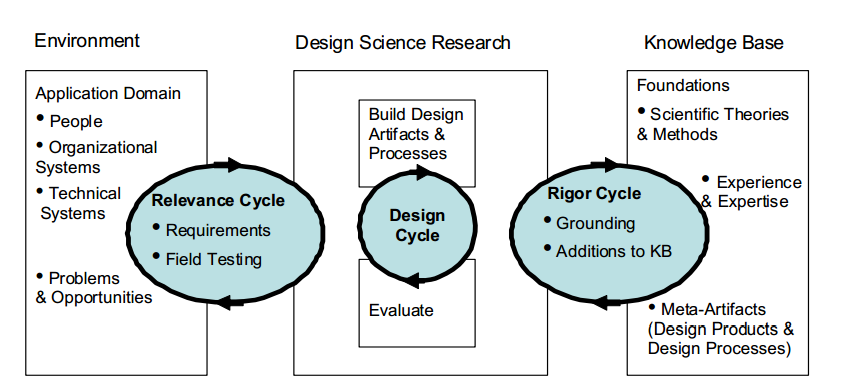
\includegraphics[width=0.4\textwidth]{Design_science.png}
	\caption{Design Science}
	\label{fig:design} %always place your label after your caption!
\end{figure}
In the research requirements will be specified. These requirements will be gathered from existing solutions. In the research new solutions combined with existing solutions and the result of this new solution will be given. After that a conclusion will follow. 

\section{Research approach}
\begin{figure}[H]
	\centering 
	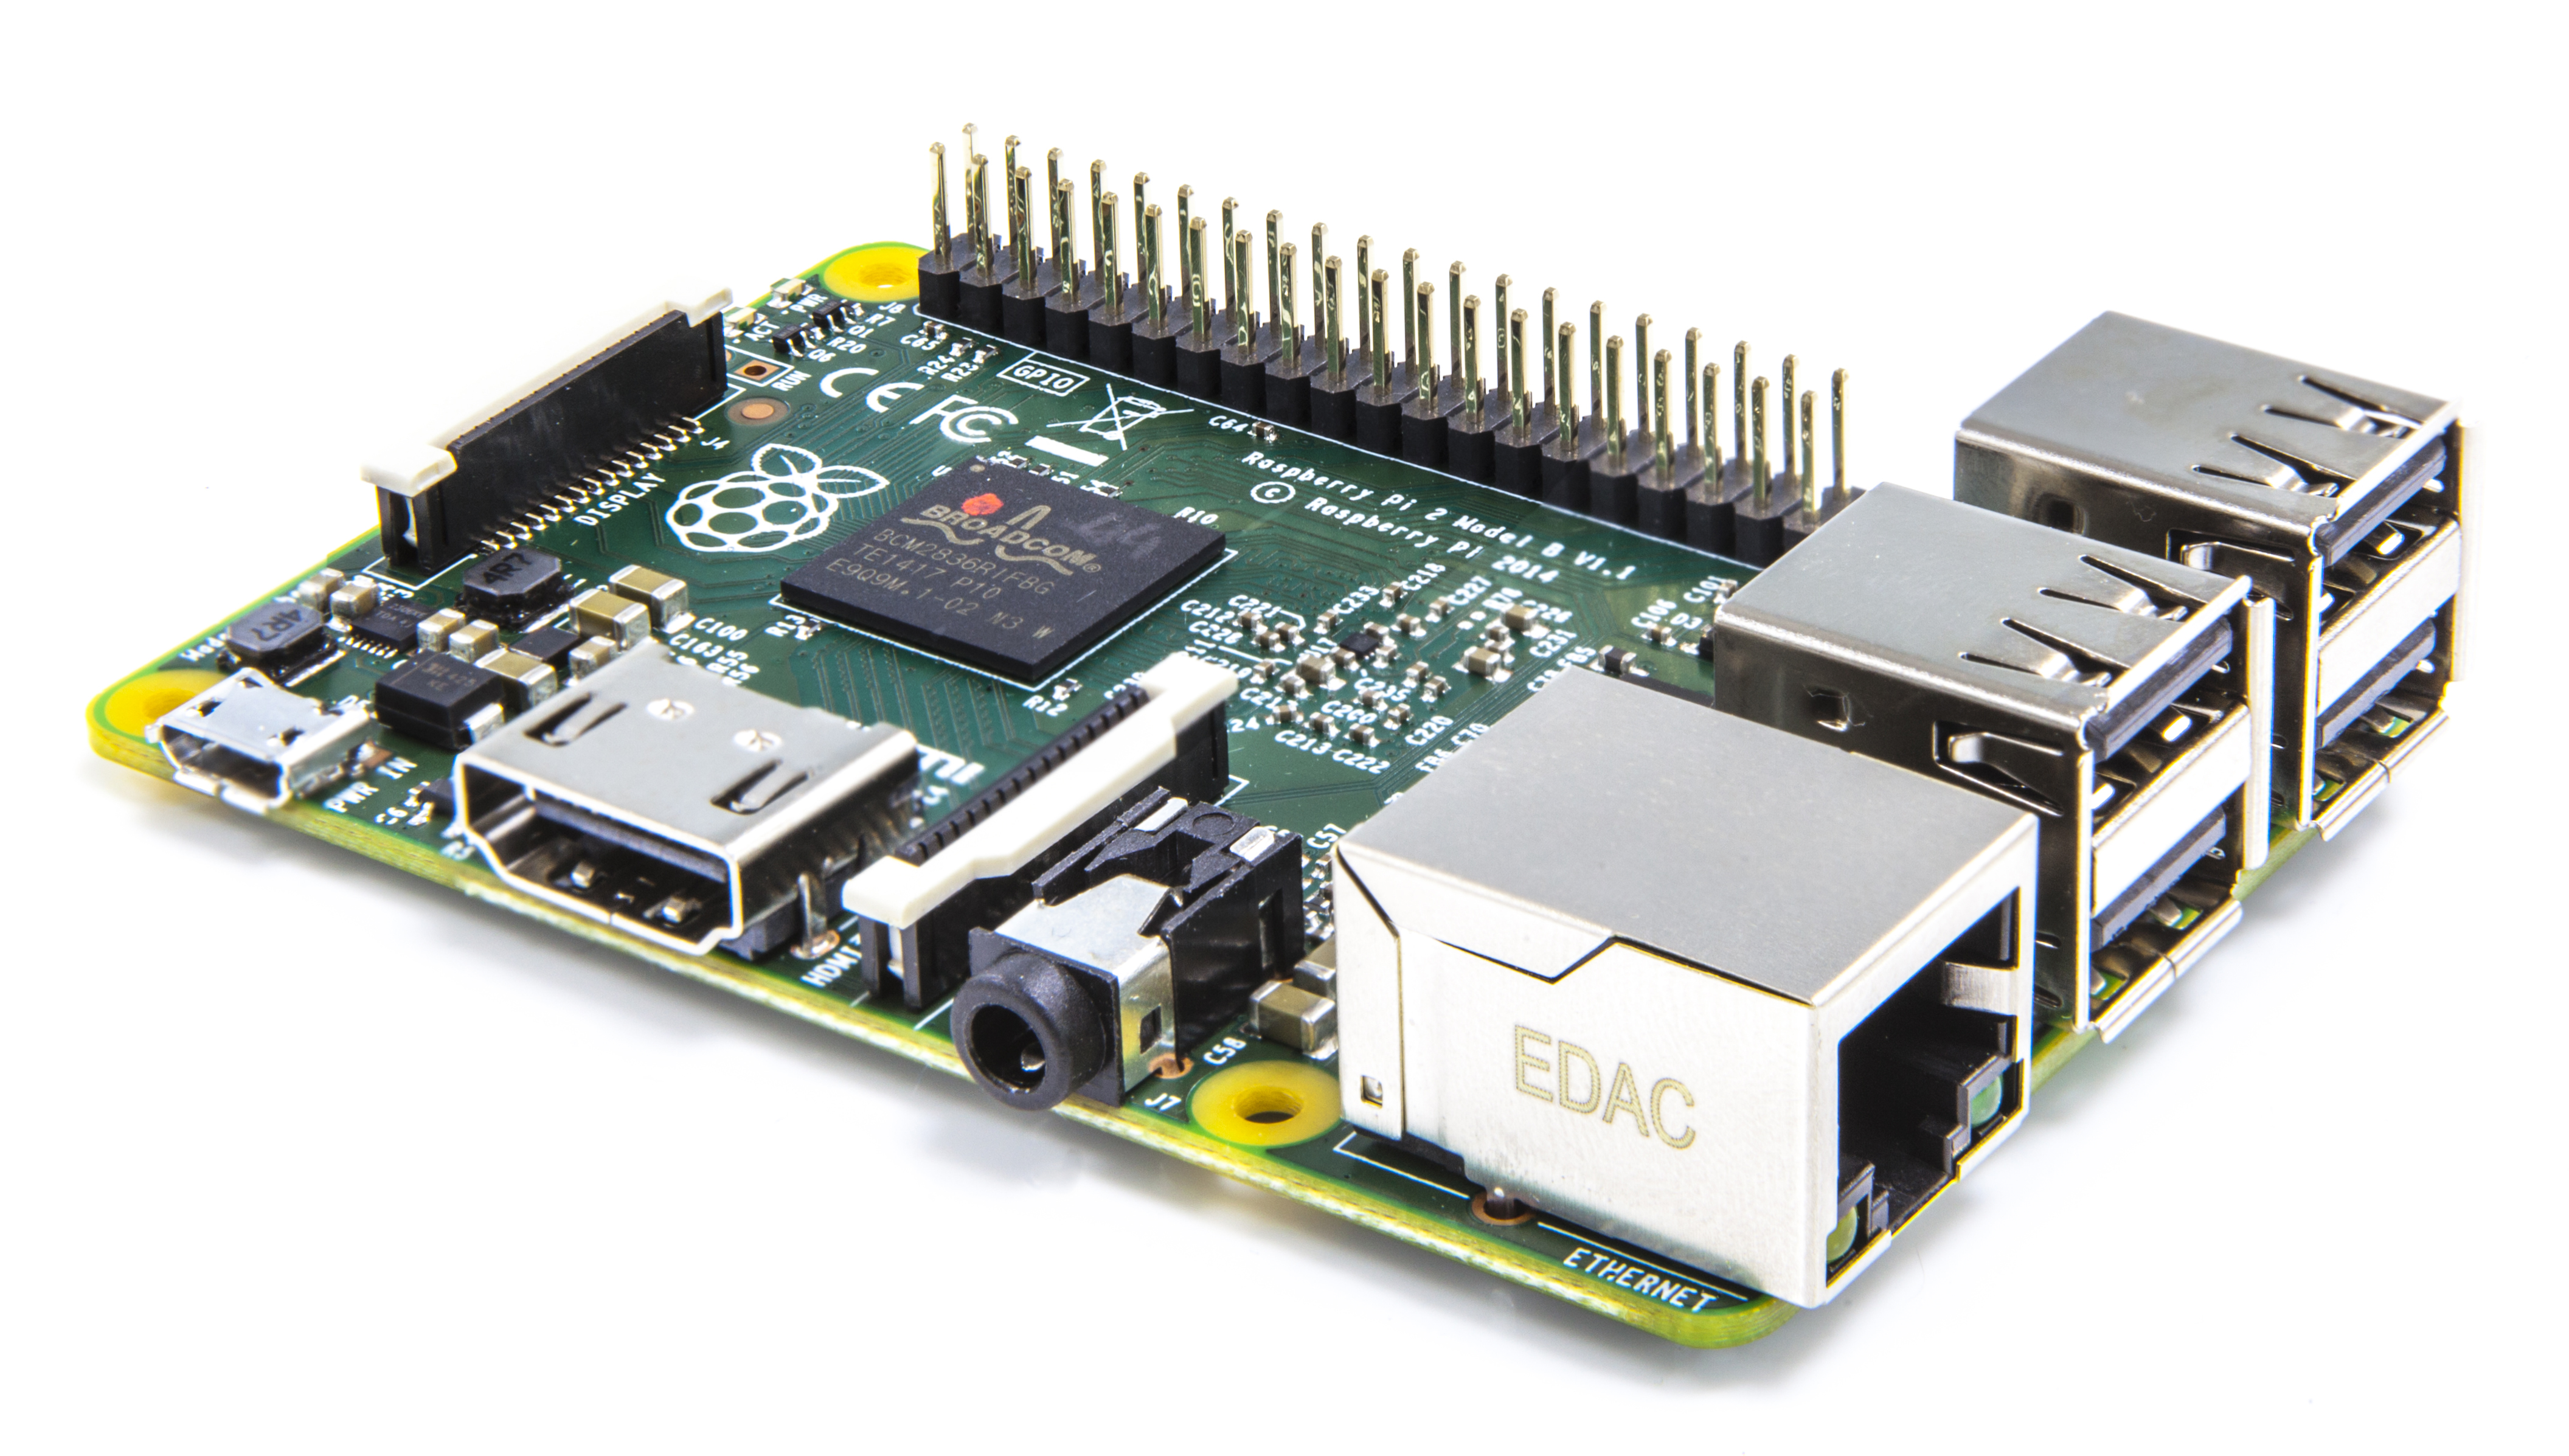
\includegraphics[width=0.4\textwidth]{Pi2ModB1GB_-comp.jpeg}
	\caption{Raspberry Pi 2 model B}
	\label{fig:raspberry} %always place your label after your caption!
\end{figure}
\begin{table}[H]
	\centering \caption{Specificaties}
	\begin{tabular}{|c|c|} \hline
		Ethernet & 100 MBps \\ \hline
		USB & 4 x USB 2.0 \\ \hline
		Video out & HDMI 1.4 \\ \hline
		Audio & 2 x analog \\ \hline
		CPU & 900MHz quad-core ARM Cortex-A7 \\ \hline
		card slot & Micro SD  \\ \hline
	\end{tabular}
	\label{tab:Specificaties}
\end{table}
For the experiment we need a Raspberry Pi 2 that can make use of the Ethernet. This is because a Raspberry Pi can be used as a webserver and this is needed in order to make video streaming possible. Beside the Raspberry Pi a several other things will be needed. For this we have a cost structure. You can view the cost structure in the appendix. \newline
So first the video streaming webserver will be made. 
After this we will make a cluster with one Raspberry Pi as a load balancer and the others as a video stream pi.  For the video streaming performance several tests can be done. For example some test in streaming in different quality with load balancing. 

\begin{figure}[H]
\centering 
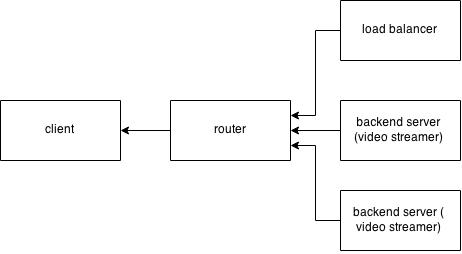
\includegraphics[width=0.4\textwidth]{raspberry pi setup.jpg}
\caption{Setup}
\label{fig:setup} %always place your label after your caption!
\end{figure}
The setup of the Raspberry Pi can be seen in the figure above ~\ref{fig:setup}.


\section{Planning}

\begin{table}[H]
	\centering \caption{Planning}
\begin{tabular}{|c|c|c|} \hline
		\textbf{Week} & \textbf{Start Date} & \textbf{Activity} \\ \hline 
		6-13& 6 Feb& Collect literature and software\\ \hline 	
		14& 23-30 March & \textbf{Deadline proposal} \\ \hline
		16 & 1 April &  \textbf{Accept Reject proposal} \\ \hline
		April May& 6 March& Building test environment \\ \hline
		16& 12 April & Answer subquestion 1  \\ \hline
		17& 21 April & Answer subquestion 2\\ \hline
		18& 27 April & Answer subquestion 3\\ \hline		
		20& 11 May  & Answer subquestion 4 \\ \hline
		21& 18 May & conclusion and check coherency \\ \hline
		21-22& 18 May & Finalize paper \\ \hline
		22& 1 June &  \textbf{Deadline paper} \\ \hline
		23& 8 June & Peer review \\ \hline
		24-25& 15 June & presentation preparation \\ \hline
		26 & 22 June & \textbf{Conference} \\ \hline
		\end{tabular}

		\label{tab:planning}
\end{table}
Here above is the table~\ref{tab:planning}. The main research question is split up into several sub questions. These subquestions have each one week for answering. After that there is time to write the conclusion and answer the main question. Then there is still some time left to finalize the paper and make the presentation. 

\section{State of the Art}
Today most of us have some data in the cloud. But Despite the attention
from the research community, research and development of
Cloud Computing services is still in it's early days~\cite{tso:2013}.Cloud computing is  the trend that IT moves data away from desktop and portable PCs into large data centers \cite{dikaiakos:2009}. Customers want to have everything has to be accessible through the network around the clock \cite{youseff:2008}. One thing that people want on demand are there film series. Currently Netflix has 30\% of the data downstream in the United States~\cite{computer-networking}. This data downstream is high. To make the video on demand service like Netflix possible they use servers. On these data servers a lot of improvements can be made \cite{bennett2007netflix,abrahamsson:2013,beloglazov:2010}. 

The Raspberry Pi is made for research and education purposes \cite{raspberry-pi}. The Raspberry Pi is a low cost device costing around 40 euro. It has a power consumption of only three watt and has for the price a processor that is well equipped to execute small tasks.  The Raspberry Pi is a small device and is excellent for a lot of small devices in a relatively small place. The Raspberry Pi doesn't use cooling and it can be used for very rapid elasticity and on-demand self-service. Because of it's cooling features and low power consumption compared to a normal server it might be a good alternative for the nowadays high power consuming data centers. The Raspberry Pi is really small so it seems to be a lot easier to place extra Pi in a data center. 

In this research we will make a small Raspberry Pi cloud to do research on video streaming using HTTP. This will be done using the design Science method proposed by Hevner~\cite{hevner:2007}. This research will try to find out if the Raspberry Pi performs good enough to serve as a micro cloud to be a suitable streamer to multiple web clients. The load balancing techniques that can be used for this will also be researched. The research on this cloud can help the scientific world. This because everything will be at one place which is in many cloud projects not the case. Besides that the information about what processes are running on the Raspberry Pi are well defined. In this way we can take a better look at algorithms used in video streaming and cloud performance. 

\bibliographystyle{abbrv}
\bibliography{sigproc}  % sigproc.bib is the name of the Bibliography in this case
% You must have a proper ".bib" file
%  and remember to run:
% latex bibtex latex latex
% to resolve all references
%
% ACM needs 'a single self-contained file'!
%
\vspace{50 mm}
\newpage
%APPENDICES are optional
\appendix
\section{Cost structure}
\begin{figure}[H]
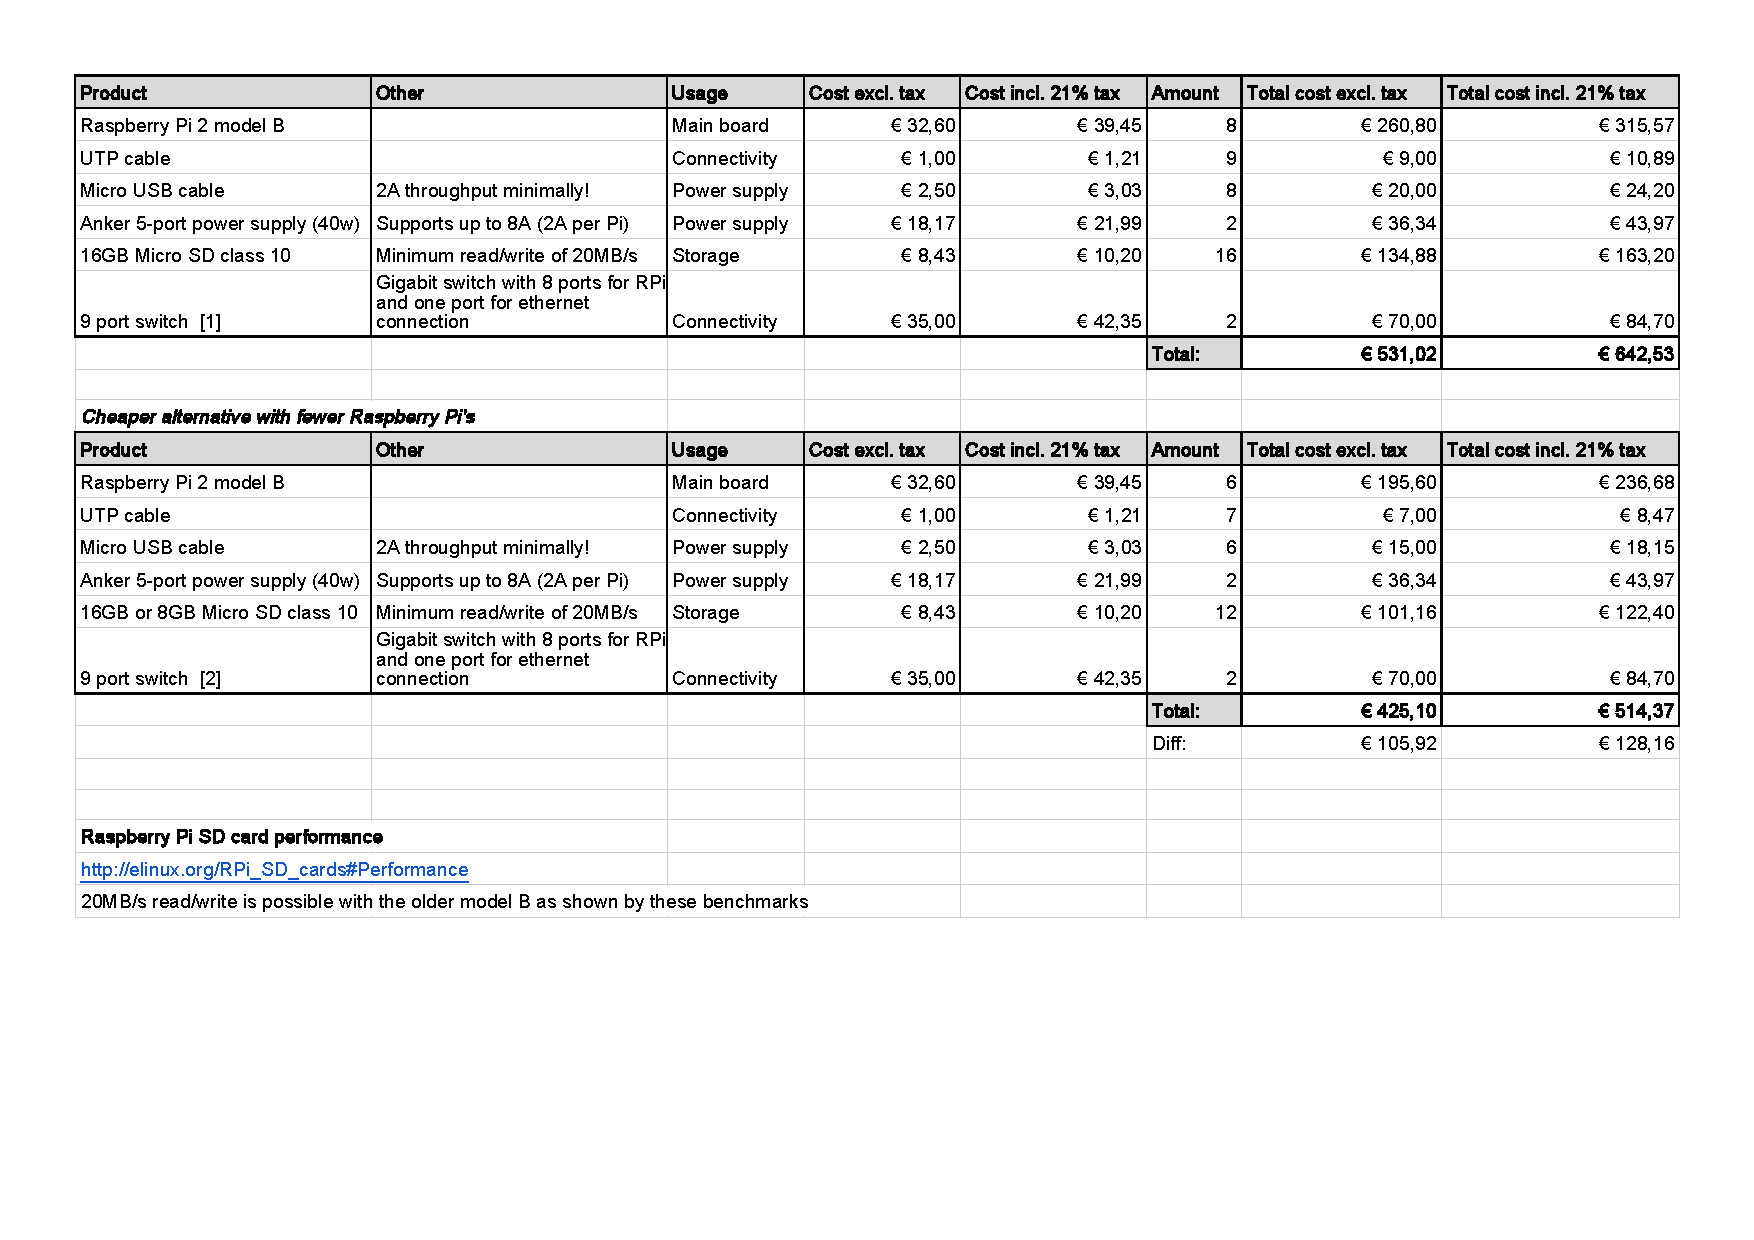
\includegraphics[scale=0.65]{Kostenoverzicht_cluster.pdf}
\label{fig:cost}
\caption{Cost structure}
\end{figure}
\end{document}
